\begin{figure*}[h]
	\centering
	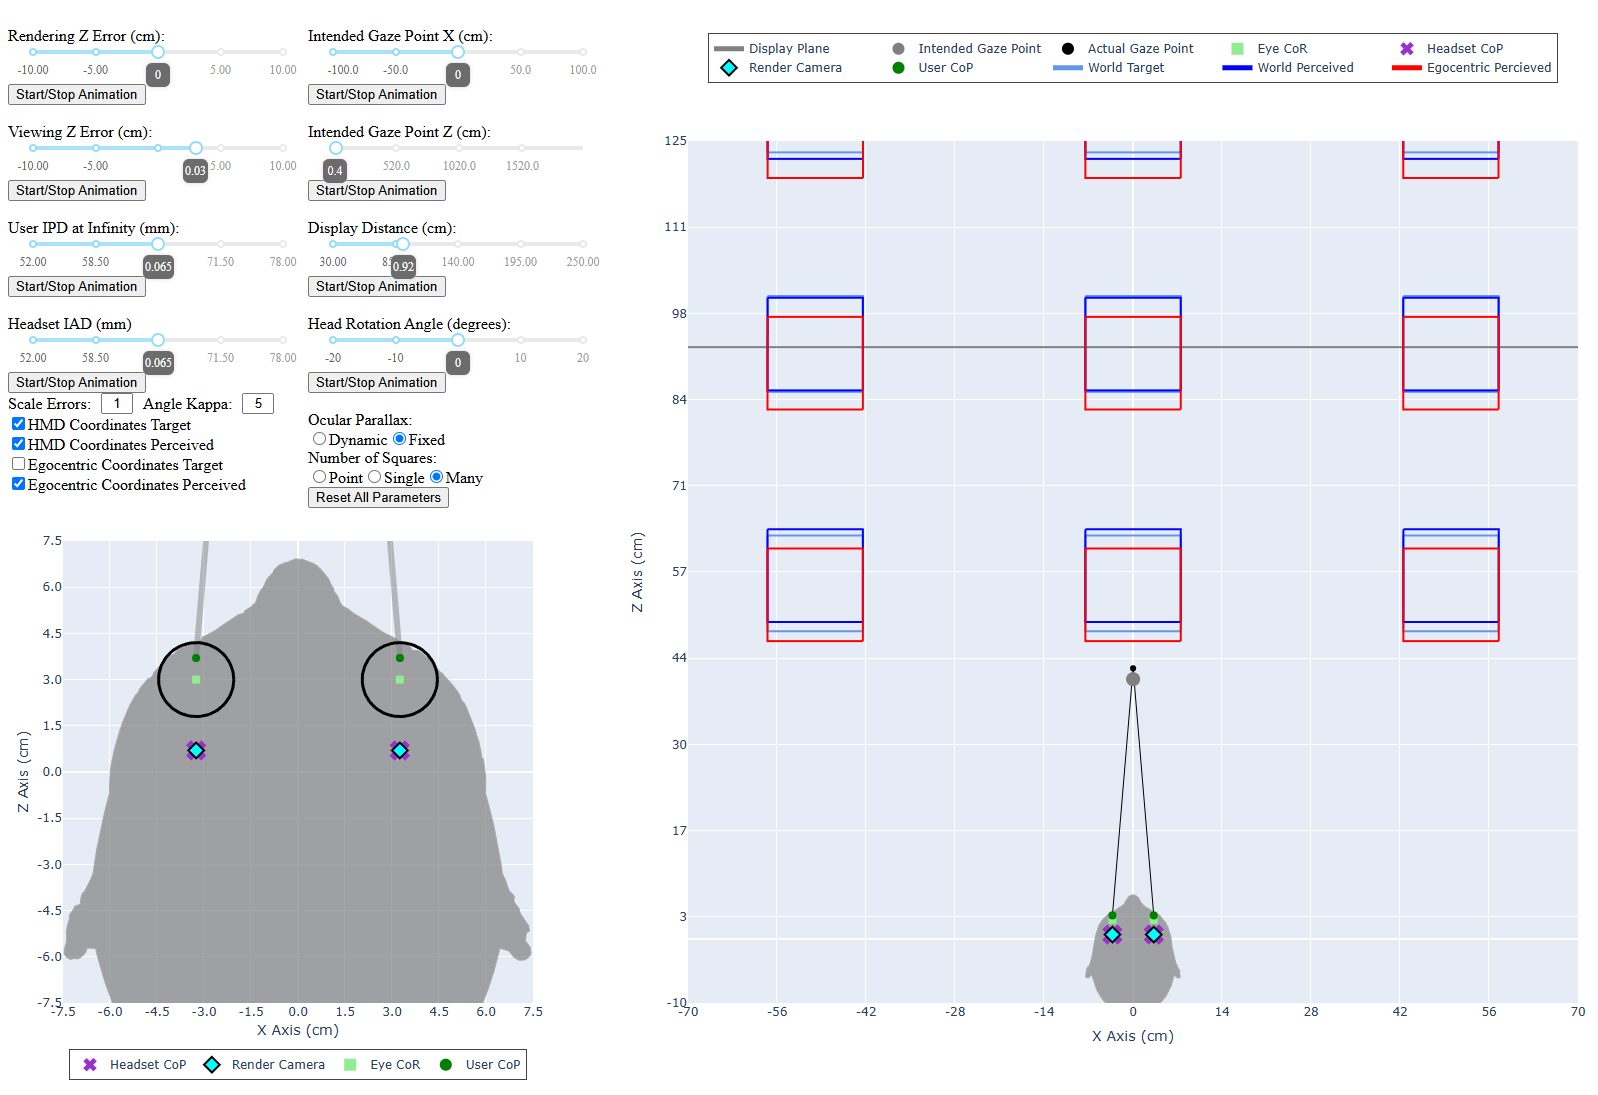
\includegraphics[width=\linewidth]{figures/model/webapp.png}    
	\caption{Interactive perspective stereo geometry visualizer provided in supplementary materials. In this simulation a viewing error moves the viewer 3 cm forward relative to the HMD coordinate system which leads to a 3 cm offset between the egocentric and HMD coordinate systems. This leads to potential discrepancies in conclusions about perceived distance if measurements taken in these two coordinate systems are directly compared. The intended render geometry in the HMD coordinate system is shown in light blue. The perceived geometry in HMD coordinate system according to perspective geometry is shown in dark blue. For viewing errors, objects on the virtual image plane are always perceived to be on the plane, according to stereo geometry. This means the center row of objects will appear near their intended position. However, because the viewer is closer to the display by 3 cm, this means that they will perceive the objects to be closer to them by 3 cm (boundaries in red) compared to the assumed HMD render geometry. This difference in coordinate systems can lead to seemingly paradoxical situations. For the row of objects closet to the user, the user will blind reach to the dark blue boundary, leading an external observer to think distance is overestimated (compared to light blue target). Yet the actual perception of the user is the red boundary and distance is in fact underestimated.} 
	\label{fig:geometric_model}
\end{figure*}

\begin{figure*}
	\centering
	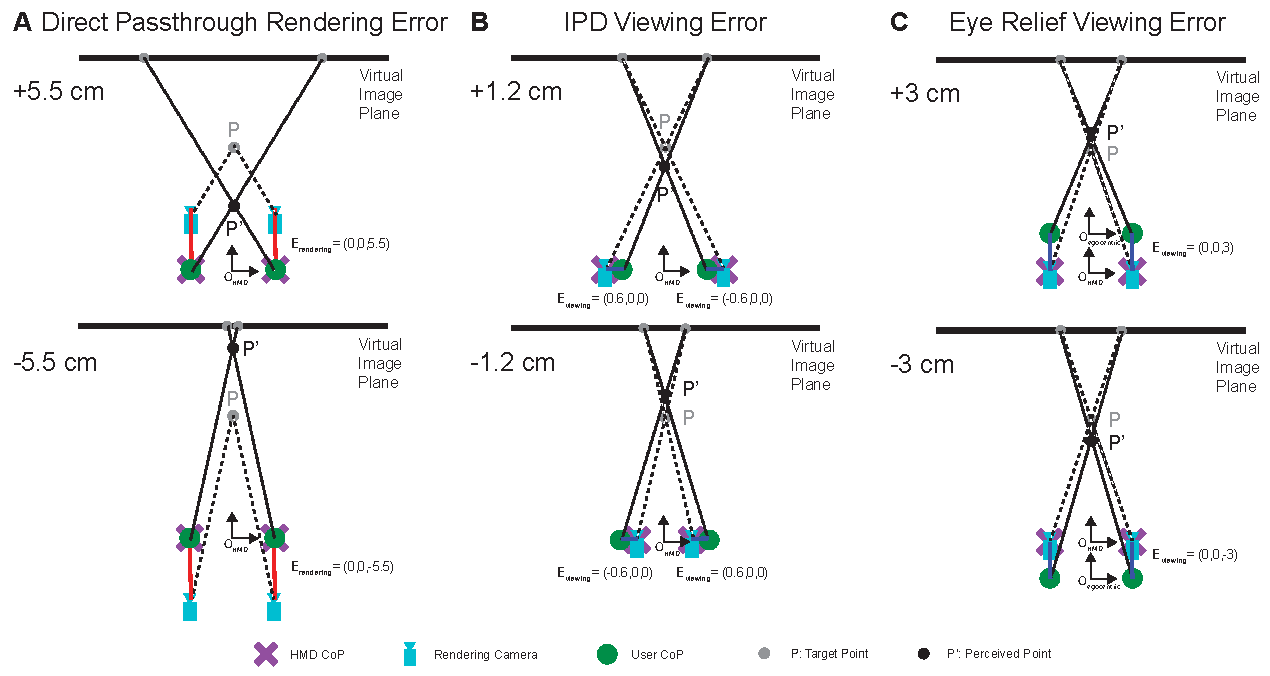
\includegraphics[width=\linewidth]{figures/reaching/error_choices.pdf}
	\caption{Rendering and viewing error conditions for the blind reaching experiments. \textbf{(A)} Direct passthrough rendering error results from showing images of cameras attached to the front of HMD without view reprojection. \textbf{(B)} IPD viewing error occurs when interaxial distance (IAD) of the HMD is smaller or larger than the user IPD. \textbf{(C)}. Eye relief viewing error is due to user's eyes being in front or behind the HMD CoP due to facial geometry. 
	}
	\label{fig:error_choices}
\end{figure*}


% \begin{figure*}
% 	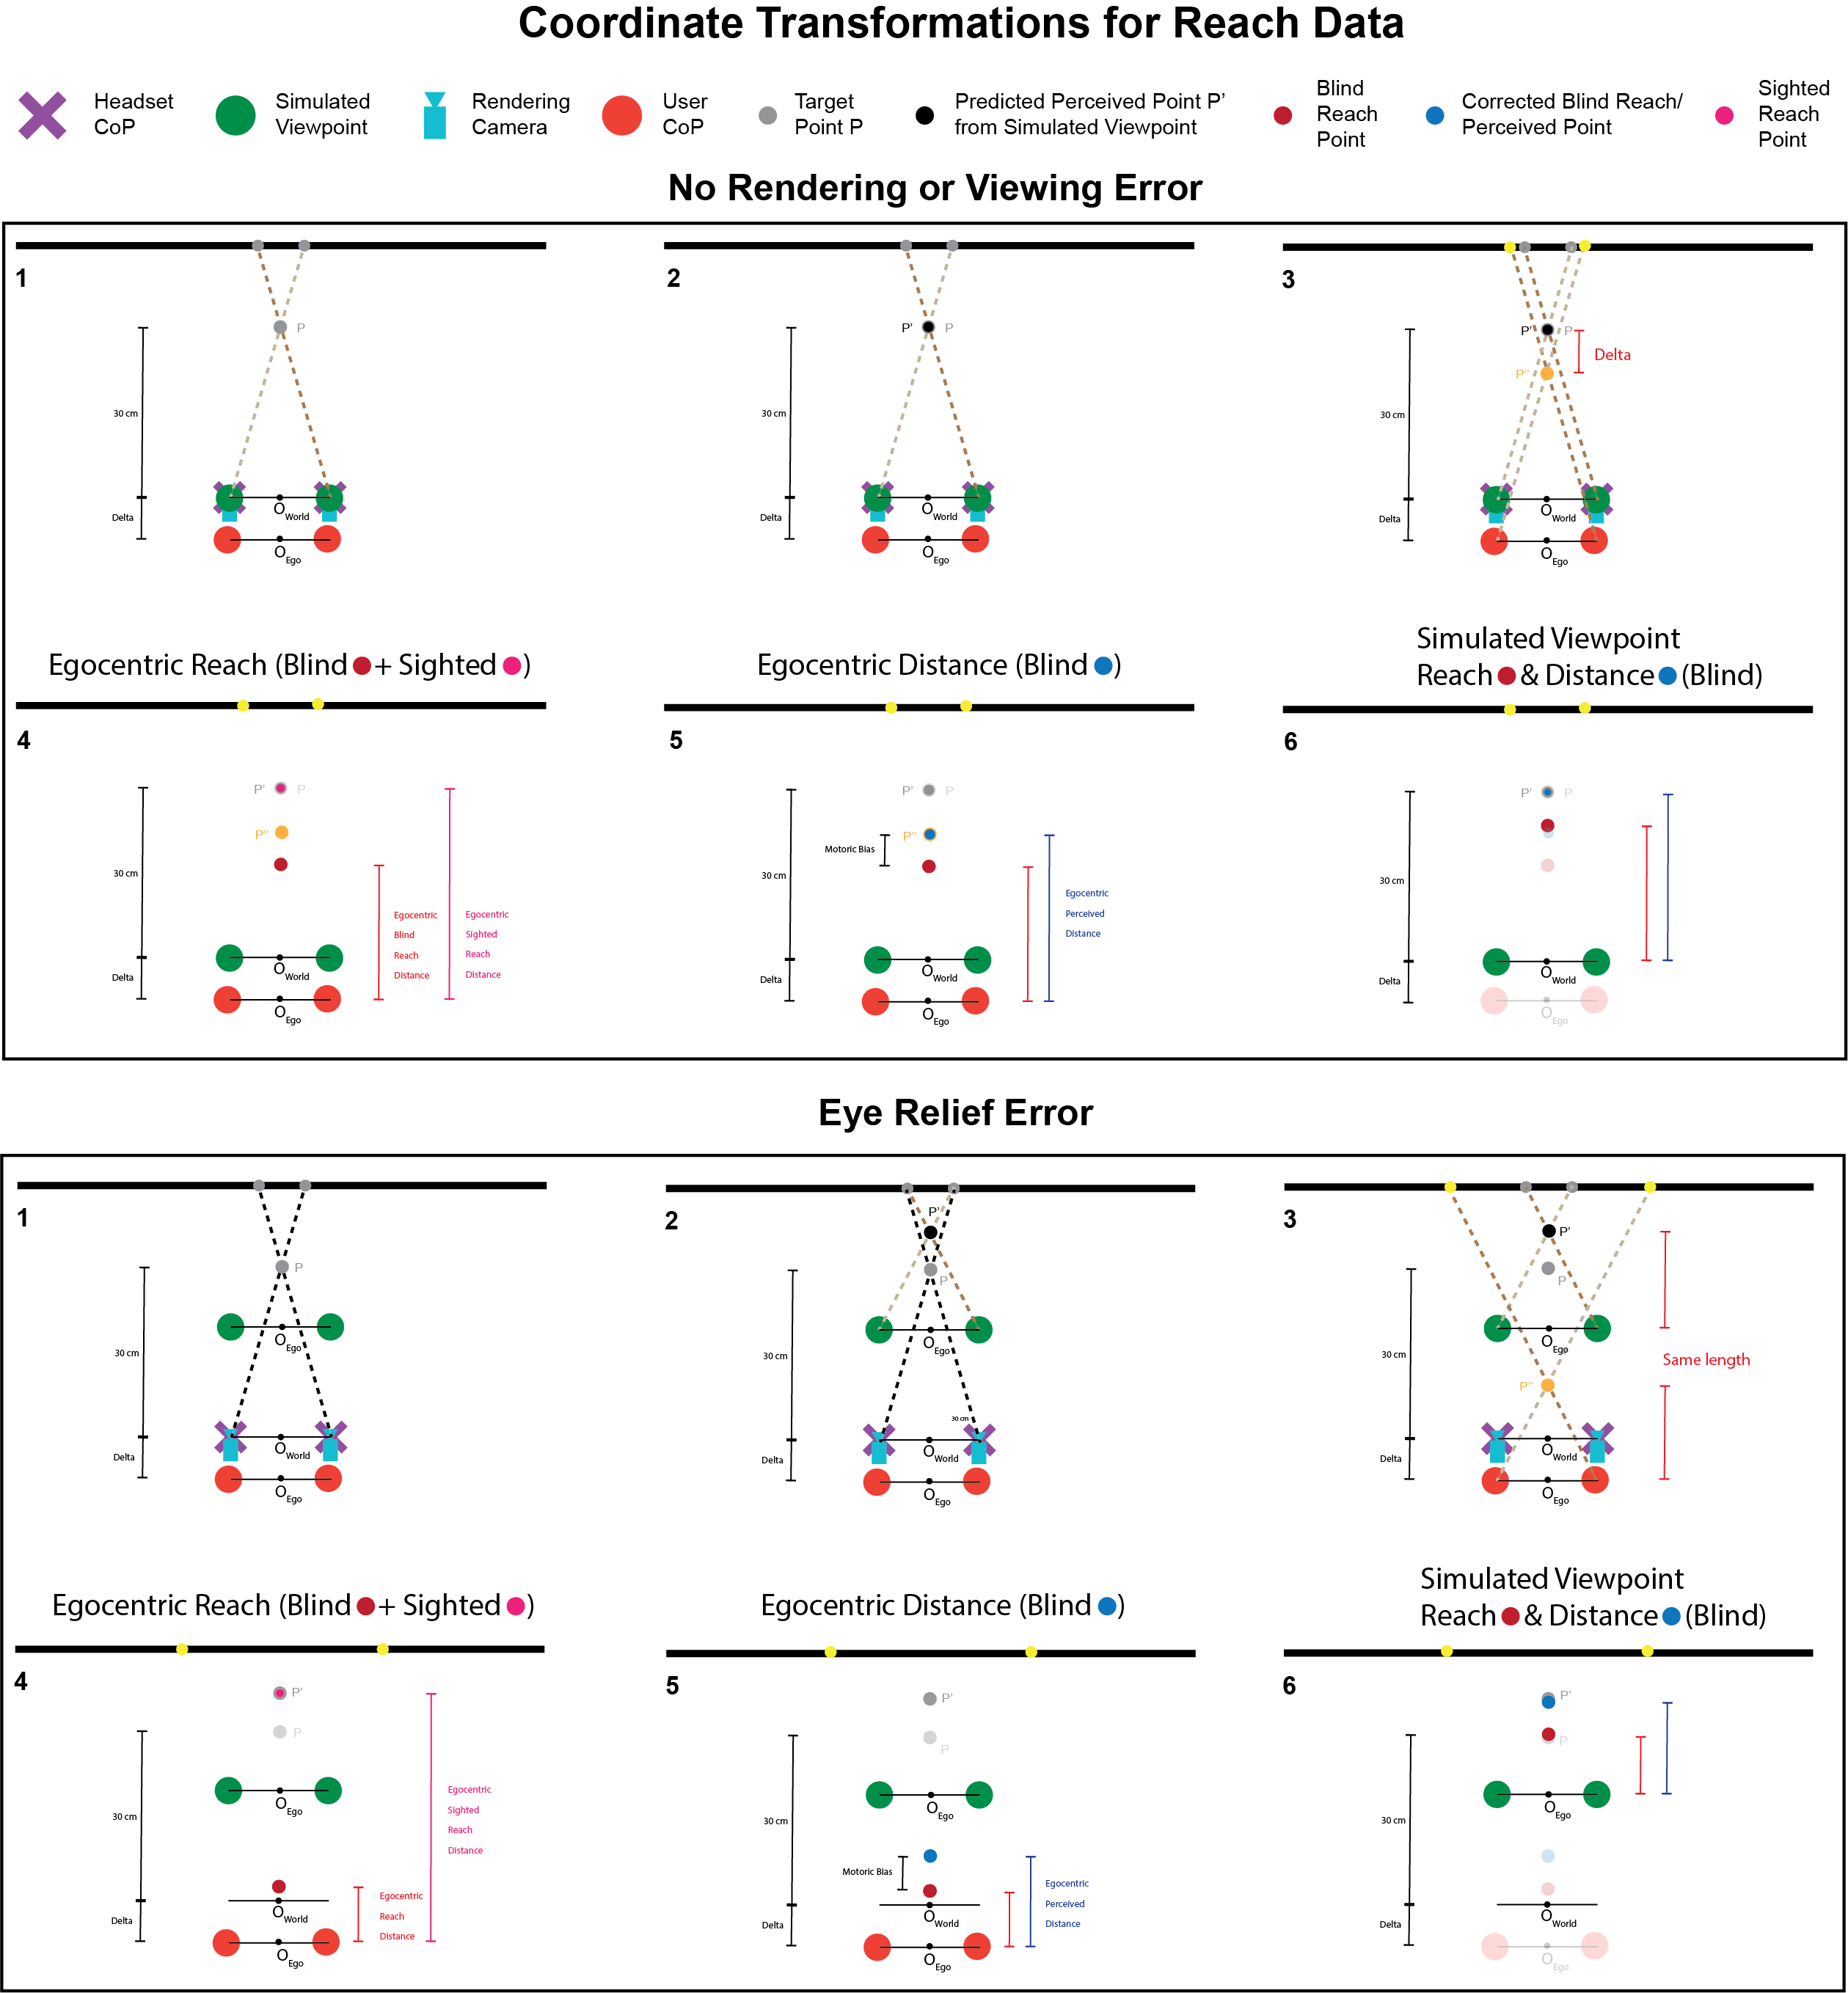
\includegraphics[width=1\textwidth]{figures/model/world_vs_egocentric_frame_step_by_step_combined.png}
%         \caption{Coordinate system transforms used to interpret reaching data studies. \textbf{(Top)} Our headset uses the largest Quest 3 eye relief setting available which results in an average eye relief viewing error of -12 mm. In panels 1-2 we show how a target point P is rendered at P' when no stereo geometry errors are added to the system. In panel 3 the rays used to simulated viewpoint are shown to the actual user who is slightly displaced away from the ideal eye relief resulting in a perceived point P'. In panels 4-6 we describe how sighted reaching, blind reaching, and bias-corrected blind reaching can be converted from measured values into their equivalent perceived values based on the small offset delta between the actual user eye position and simulated viewpoint. \textbf{(Bottom)} Simulated eye relief viewing errors require another transform to interpret egocentric reach data in the simulated viewpoint HMD coordinates which is shown in panels 5 and 6.}
% 	\label{fig:simulation_geometry}
% \end{figure*}

% \begin{figure*}
% 	\includegraphics[width=1\textwidth]{figures/model/distortion_field.png}
%         \caption{Geometric distortion fields in world coordinates at errors used in reaching experiments. \textbf{(A,B)} Direct passthrough errors. \textbf{(C,D)} Eye relief viewing error error. \textbf{(E,F)} mismatched IPD-IAD errors. For viewing errors (C-F), points on the virtual image plane are not distorted. For rendering errors (A-B), distortions are the same irrespective of virtual image plane distance.}
% 	\label{fig:distortion_vector_field_summary}
% \end{figure*}

